\documentclass[tikz, border=5mm]{standalone}
\usepackage{amsmath}
\usepackage{graphicx} % Necesario para importar la imagen de Fashion MNIST
\usetikzlibrary{calc, arrows.meta, positioning, decorations.pathreplacing} 

\begin{document}
\begin{tikzpicture}[
    % Estilos globales
    arrow line/.style={->, >=Stealth, thick, dashed, color=black!50},
    title style/.style={font=\bfseries\small, align=center}
]

    % =========================================================================
    % CUADRO 1 (Izquierda): Datos Originales (Fashion MNIST)
    % =========================================================================
    \begin{scope}[xshift=0cm, yshift=0cm]
        \node[title style, color=blue!80!black] at (1.5, 4.5) {Datos Originales};
        
        % Contenedor exterior
        \draw[draw=black!30, fill=gray!5, rounded corners] (0, 0) rectangle (3, 4);

        % Importación de la imagen de Fashion MNIST
        % (Asegúrate de tener 'dataset-cover.png' en el mismo directorio)
        \node[inner sep=0pt] (fmnist) at (1.5, 2.0) {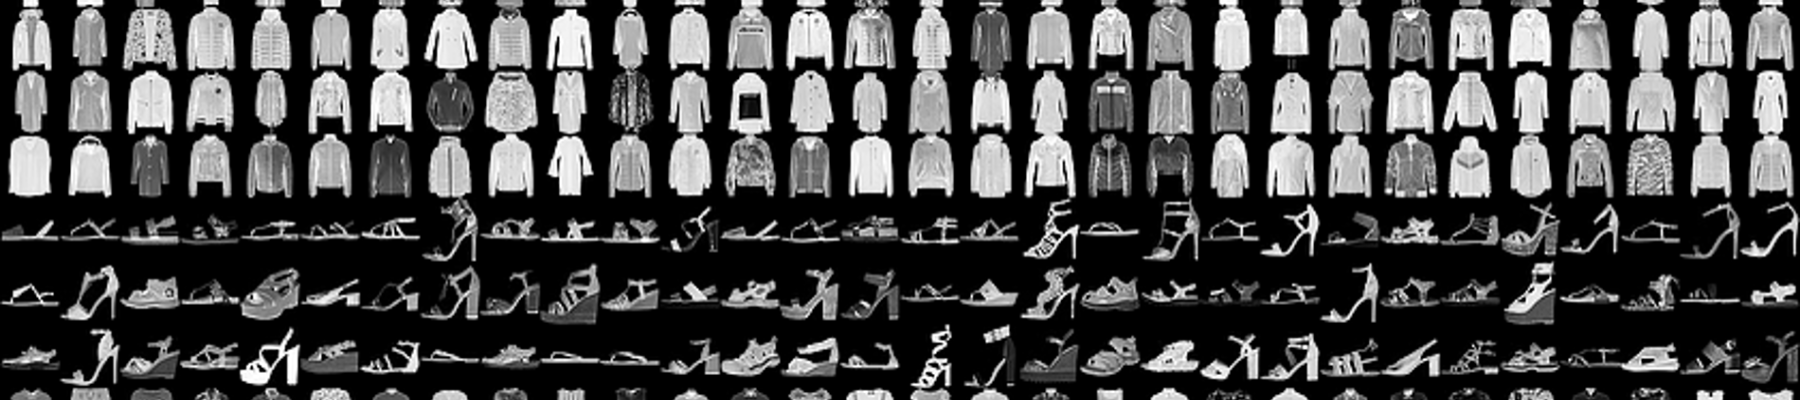
\includegraphics[width=5.5cm, trim=8in 0 5.5in 0, clip]{dataset-cover.png}};

        % Puntos u y v superpuestos sobre la imagen
        \coordinate (itemU) at (1.2, 3.1);
        \coordinate (itemV) at (1.9, 0.9);
        
        % Se agrega un fondo blanco al texto para que sea legible sobre la imagen
        \fill[red] (itemU) circle (2.5pt) node[above=2pt, font=\tiny\bfseries, fill=white, inner sep=1.5pt, rounded corners=1pt] {$u$};
        \fill[red] (itemV) circle (2.5pt) node[below=2pt, font=\tiny\bfseries, fill=white, inner sep=1.5pt, rounded corners=1pt] {$v$};
    \end{scope}

    % =========================================================================
    % CUADRO 2 (Centro): Funciones LSH (Retículas Infinitas)
    % =========================================================================
    \begin{scope}[xshift=5.0cm, yshift=0cm]
        \node[title style, color=orange!80!black] at (2.0, 4.5) {Funciones LSH};
        
        % Contenedor exterior (Fondo)
        \draw[draw=black!30, fill=gray!5, rounded corners] (0, 0) rectangle (4, 4);

        % --- INICIO DEL CLIPPING ---
        % Todo lo que se dibuje dentro de este 'scope' será recortado a los bordes del cuadro
        \begin{scope}
            \clip[rounded corners] (0, 0) rectangle (4, 4);

            % Dibujamos retículas desde -10 hasta 10 para garantizar que cubran todo el encuadre
            
            % Retícula 1: Base (Color Gris Suave)
            \begin{scope}[opacity=0.4, color=gray, x={(0.5cm,0.2cm)}, y={(0.2cm,0.6cm)}]
                \foreach \x in {-10,...,10} \draw[densely dashed] (\x,-10) -- (\x,10);
                \foreach \y in {-10,...,10} \draw[densely dashed] (-10,\y) -- (10,\y);
            \end{scope}

            % Retícula 2: Desplazada y Rotada (Color Celeste)
            \begin{scope}[opacity=0.5, color=cyan!70!black, x={(0.45cm,-0.15cm)}, y={(0.25cm,0.55cm)}]
                \foreach \x in {-10,...,15} \draw[dashed] (\x,-10) -- (\x,10);
                \foreach \y in {-10,...,10} \draw[dashed] (-10,\y) -- (15,\y);
            \end{scope}

            % Retícula 3: Mayor rotación (Color Púrpura)
            \begin{scope}[opacity=0.6, color=purple!60, x={(0.35cm,0.3cm)}, y={(-0.2cm,0.5cm)}]
                \foreach \x in {-10,...,10} \draw[densely dashed, thick] (\x,-10) -- (\x,15);
                \foreach \y in {-10,...,15} \draw[densely dashed, thick] (-10,\y) -- (10,\y);
            \end{scope}
        \end{scope}
        % --- FIN DEL CLIPPING ---

        % Borde superior para rematar el cuadro (ya que el clip a veces muerde la línea original)
        \draw[draw=black!30, rounded corners] (0, 0) rectangle (4, 4);

        % Nodos de proyección interna donde intersectan las características
        \coordinate (midU) at (1.8, 2.8);
        \coordinate (midV) at (2.4, 1.6);
        
        % Fondo blanco en etiquetas para que las retículas no estorben la lectura
        \fill[red] (midU) circle (2pt) node[above right=1pt, font=\tiny\bfseries, color=black, fill=white, inner sep=1pt] {$g(u)$};
        \fill[red] (midV) circle (2pt) node[below left=1pt, font=\tiny\bfseries, color=black, fill=white, inner sep=1pt] {$g(v)$};
    \end{scope}

    % =========================================================================
    % CUADRO 3 (Derecha): Tabla LSH (Cubetas de colisión indexadas)
    % =========================================================================
    \begin{scope}[xshift=11.0cm, yshift=0cm]
        \node[title style, color=green!50!black] at (1.0, 4.5) {Tabla LSH};
        
        % Contenedor exterior
        \draw[draw=black!30, fill=gray!5, rounded corners] (0, 0) rectangle (2, 4);

        % Renderizado de la tabla densa (Cadena de celdas delgadas de 0.25cm de alto)
        \foreach \s in {0,...,14} {
            \draw[draw=black!40, fill=white] (0.4, \s*0.25 + 0.1) rectangle (1.6, \s*0.25 + 0.35);
        }

        % Definición de los buckets de destino
        \coordinate (dstU) at (0.4, 11*0.25 + 0.22); % Cubeta asignada a u
        \coordinate (dstV) at (0.4, 4*0.25 + 0.22);  % Cubeta asignada a v
    \end{scope}

    % =========================================================================
    % CONEXIONES CURVADAS INTER-PANEL (Mapeo de Flujo)
    % =========================================================================
    
    % --- Flujo del Ítem U ---
    \draw[arrow line] (itemU) to [out=15, in=165] (midU);
    \draw[arrow line] (midU) to [out=10, in=180] (dstU);
    \fill[red] (dstU) circle (2pt) node[right=1pt, font=\tiny\bfseries] {$u'$};

    % --- Flujo del Ítem V ---
    \draw[arrow line] (itemV) to [out=0, in=195] (midV);
    \draw[arrow line] (midV) to [out=-15, in=180] (dstV);
    \fill[red] (dstV) circle (2pt) node[right=1pt, font=\tiny\bfseries] {$v'$};

\end{tikzpicture}
\end{document}

